\section{Neutronenbombe}
\begin{frame}
	\begin{block}{Die Neutronenbombe}
	\end{block}
\end{frame}
\begin{frame}{Samuel T. Cohen}
	\begin{columns}[onlytextwidth]
		\begin{column}{0.45\textwidth}
			\begin{itemize}
				\item 25.01.1921 - 28.11.2010
				\item "Vater der Neutronenbombe"
				\item Berechnete das Neutronenverhalten von Fat Man
				\item wollte "a clean Bomb" entwickeln
			\end{itemize}
		\end{column}
		\begin{column}{0.45\textwidth}
			\begin{figure}
				\centering
				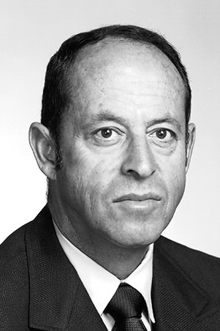
\includegraphics[width=0.5\textwidth]{img/samuel_cohen.jpg}
				\caption{Samuel T. Cohen \cite{JewCurr}}
			\end{figure}
		\end{column}
	\end{columns}
\end{frame}
\begin{frame}{Idee}
	\begin{itemize}
		\item Soldaten sollen schnell sterben oder sich schnell erholen können
		\item das Schlachtfeld soll schnell wieder bewohnbar sein
		\item gegnerische Waffen und Befestigungen zur Eigennutzung erhalten
	\end{itemize}
\end{frame}
\begin{frame}{Funktion}
	\begin{itemize}
		\item Fusionsbombe mit "invertiertem" Wirkungsgrad
		\item \begin{description}
						\item[Fusionsbombe] 50\,\% Druckwelle, 35\,\% thermische Strahlung, 15\,\% Strahlung
						\item[Neutronenbombe] 30\,\% Druckwelle, 20\,\% thermische Strahlung, 50\,\% Strahlung
					\end{description}
		\item Sprengkraft von ca. \SI{1}{\kilo \tnt}
		\item letal im Radius von ca. \SI{2000}{\meter}
	\end{itemize}
	\pdfnote{Grundkonzept}
\end{frame}
\begin{frame}{Geschichte}
	\begin{description}
		\item[1958] Cohen entwirft die Neutronenbombe (NB)
		\item[1963-1970] USA testet verschiedene Typen der NB
		\item[1974] USA baut ca 120 NB des Types W66
		\item[17.11.1978] UDSSR testet testet eine NB
		\item[21.06.1980] Frankreich testet den ersten Prototypen
		\item[1981] unter Ronald Reagan werden 700 Sprengköpfe gebaut
		\item[1988] China testet seine erste NB
		\item[1999] Indien gibt an das Wissen zum Bau einer NB zu haben
		\item[~2000] Frankreich demontiert alle Sprengköpfe
		\item[1996-2003] unter Bill Clinton und George W. Bush werden alle Sprengköpfe der USA demontiert
		\item[Heute] Offiziell gibt es keine einsatzbereite NB
	\end{description}
\end{frame}
\begin{frame}{Übersicht}
	\begin{columns}[onlytextwidth]
		\begin{column}{0.45\textwidth}
			\begin{block}{Pro}
				\begin{itemize}
					\item lässt Gebäude und Infrastruktur weitgehend intakt
					\item tötet auch gepanzerte Einheiten, zB. Panzerbesatzung
					\item dringt in unterirdische Bunker ein
					\item nach 24 bis 48 Stunden ist die Radioaktivität abgeklungen
				\end{itemize}
			\end{block}
		\end{column}
		\begin{column}{0.45\textwidth}
			\begin{block}{Contra}
				\begin{itemize}
					\item Qualvoller Tod
					\item Reichweite stark von Luftfeuchtigkeit abhänig
					\item Kleinere Hemmschwelle
				\end{itemize}
			\end{block}
		\end{column}
	\end{columns}
\end{frame}
\begin{frame}{Auswirkungen}
	\begin{block}{Video}
		\begin{figure}
			\centering
			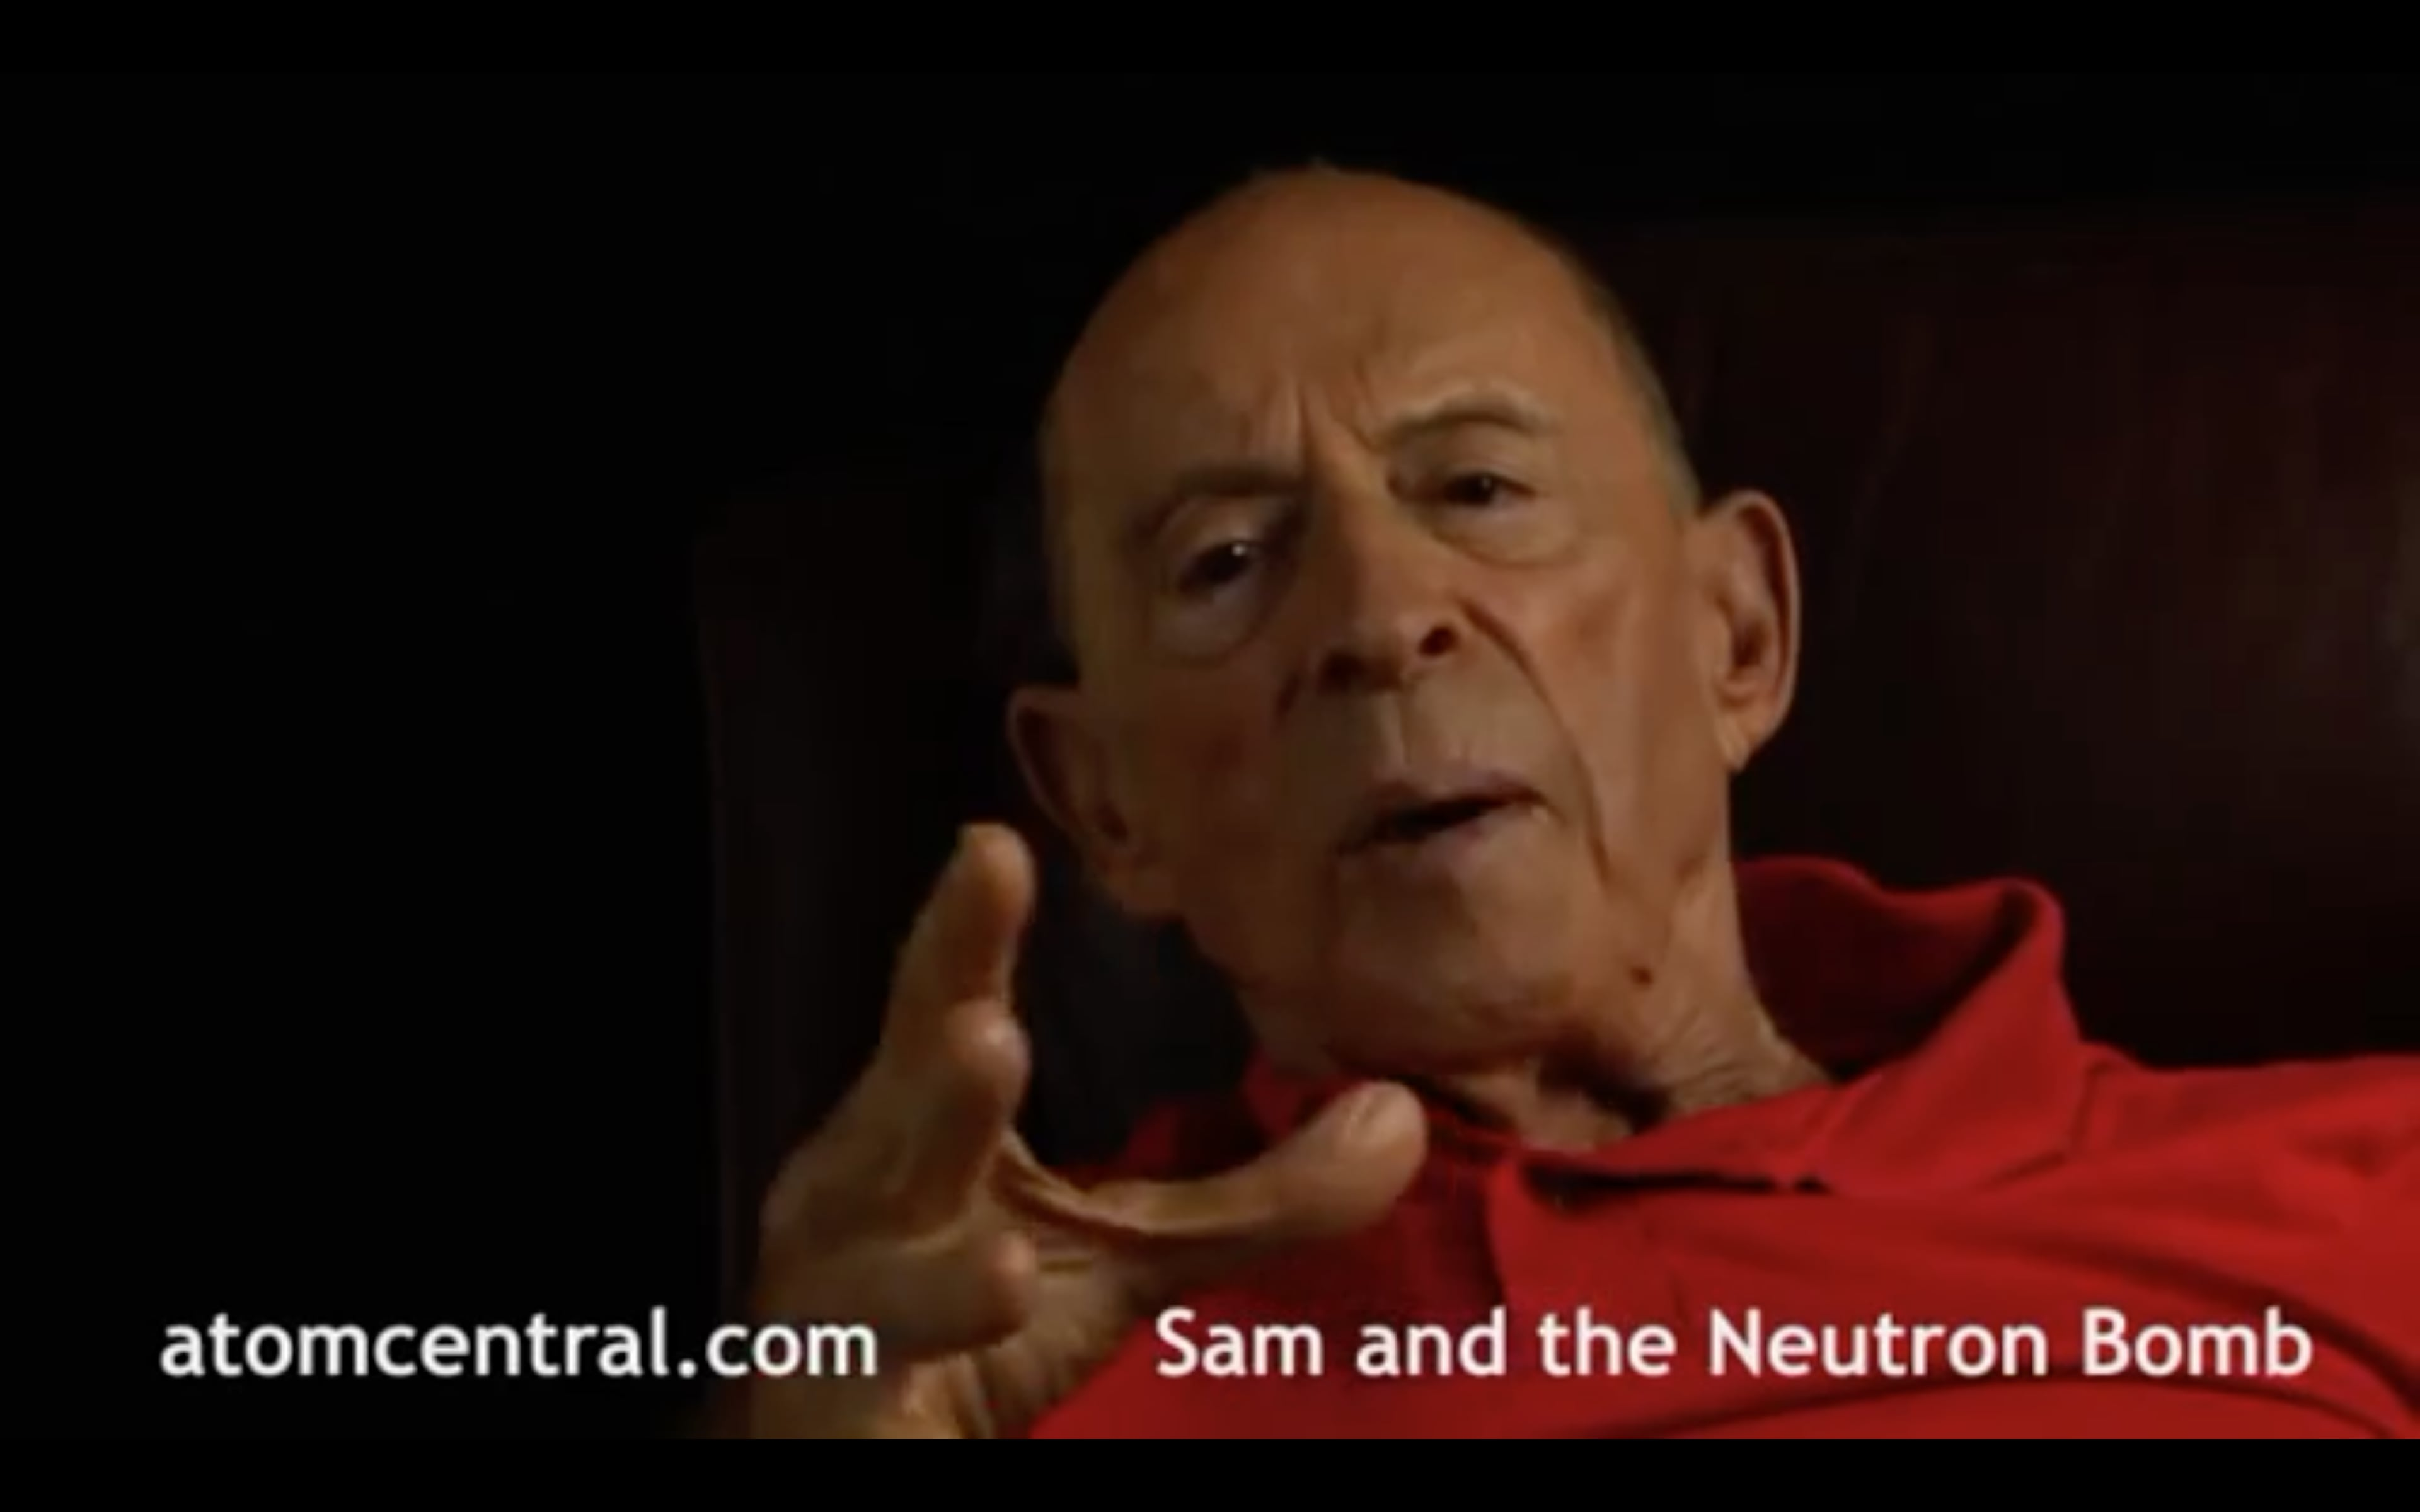
\includegraphics[width=0.5\textwidth]{img/sam_cohen_thumbnail.jpg}
			\caption{Ausschnitt von \href{https://www.youtube.com/watch?v=z_QFXGxw6Tk}{Neutron Bomb creator speaks} }
		\end{figure}
	\end{block}
\end{frame}
